

\documentclass{article}
\usepackage[utf8]{inputenc}
\usepackage[utf8]{inputenc}
\usepackage[T1]{fontenc}
\usepackage[english]{babel}
\usepackage{fullpage}
\usepackage{color}
\usepackage[table]{xcolor}
\usepackage{listings}
 
\definecolor{darkWhite}{rgb}{0.94,0.94,0.94}
 
\lstset{
  aboveskip=3mm,
  belowskip=-2mm,
  backgroundcolor=\color{darkWhite},
  basicstyle=\footnotesize,
  breakatwhitespace=false,
  breaklines=true,
  captionpos=b,
  commentstyle=\color{red},
  deletekeywords={...},
  escapeinside={\%*}{*)},
  extendedchars=true,
  framexleftmargin=16pt,
  framextopmargin=3pt,
  framexbottommargin=6pt,
  frame=tb,
  keepspaces=true,
  keywordstyle=\color{blue},
  language=C,
  literate=
  {²}{{\textsuperscript{2}}}1
  {⁴}{{\textsuperscript{4}}}1
  {⁶}{{\textsuperscript{6}}}1
  {⁸}{{\textsuperscript{8}}}1
  {€}{{\euro{}}}1
  {é}{{\'e}}1
  {è}{{\`{e}}}1
  {ê}{{\^{e}}}1
  {ë}{{\¨{e}}}1
  {É}{{\'{E}}}1
  {Ê}{{\^{E}}}1
  {û}{{\^{u}}}1
  {ù}{{\`{u}}}1
  {â}{{\^{a}}}1
  {à}{{\`{a}}}1
  {á}{{\'{a}}}1
  {ã}{{\~{a}}}1
  {Á}{{\'{A}}}1
  {Â}{{\^{A}}}1
  {Ã}{{\~{A}}}1
  {ç}{{\c{c}}}1
  {Ç}{{\c{C}}}1
  {õ}{{\~{o}}}1
  {ó}{{\'{o}}}1
  {ô}{{\^{o}}}1
  {Õ}{{\~{O}}}1
  {Ó}{{\'{O}}}1
  {Ô}{{\^{O}}}1
  {î}{{\^{i}}}1
  {Î}{{\^{I}}}1
  {í}{{\'{i}}}1
  {Í}{{\~{Í}}}1,
  morekeywords={*,...},
  numbers=left,
  numbersep=10pt,
  numberstyle=\tiny\color{black},
  rulecolor=\color{black},
  showspaces=false,
  showstringspaces=false,
  showtabs=false,
  stepnumber=1,
  stringstyle=\color{gray},
  tabsize=4,
  title=\lstname,
}
\usepackage{graphicx}
\graphicspath{ {./images/} }
\title{HAI804I – Analyse et Traitement d'Images}
\author{Fabien Caballero }

\begin{document}  

\maketitle
    \tableofcontents

\newpage

\section{Lire le fichier}
J'utilise les fonctions fopen et fread avec fopen en mode lecture binaire.
\begin{lstlisting}
   FILE *f = fopen((char *)argv[1], "rb");
    unsigned short *contenu;

    int dimX = atoi(argv[2]);
    int dimY = atoi(argv[3]);
    int dimZ = atoi(argv[4]);
    allocation_tableau(contenu, unsigned short, dimX *dimY *dimZ);

    size_t taille=fread(contenu,sizeof(unsigned short),dimX*dimY*dimZ,f);
\end{lstlisting}

Il faut penser à inverser le sens de lecture des 2 octets (MSB et LSB)
En récupérant les valeurs dans un unsigned short le LSB et MSB sont inversés.
Pour ne pas inverser il faudrait stocker chaque élément dans 2 unsigned char.
J'ai choisi les unsigned short et d'inverser.

\begin{lstlisting}
  unsigned short inverse(unsigned short val)
{
    float o1 = floor(((double)val / 256.0));
    float o2 = val - o1 * 256;

    return o2 * 256 + o1;
}
\end{lstlisting}

Une fois tout le tableau inversé, j'ai créer une fonction getValue, une max et une min.
\begin{lstlisting}

unsigned short getValue(unsigned short *img, int x, int y, int z, int dimX, int dimY, int dimZ)
{
    return (int)img[z * dimY * dimX + y * dimX + x];
}

unsigned short minElmt(unsigned short *img, size_t taille)
{
    unsigned short min = 0;
    for (size_t i = 0; i < taille; i++)
    {
        if (img[i] < min)
            min = img[i];
    }
    return min;
}

unsigned short maxElmt(unsigned short *img, size_t taille)
{
    unsigned short max = 0;
    for (size_t i = 0; i < taille; i++)
    {
        if (img[i] > max)
            max = img[i];
    }
    return max;
}

\end{lstlisting}

\newpage
J'obtient les résultats suivants:
\\\\

\textbf{t1-head}:

val(158,143,64)= 242
min= 0
max= 885

\textbf{orange}:

val(128,128,32)= 9
min= 0
max= 228


\textbf{INCISIX}:

val(184,343,83)= 1225
min= 0
max= 4095

\newpage
\section{MIP}

\begin{lstlisting}
    for (size_t i = 0; i < dimX; i++)
    {
        for (size_t j = 0; j < dimY; j++)
        {
            int max = 0;
            for (size_t k = 0; k < dimZ; k++)
            {
                if (getValue(contenu, i, j, k, dimX, dimY, dimZ) > max)
                    max = getValue(contenu, i, j, k, dimX, dimY, dimZ);
            }
            Out[j*dimX+i]=max;
        }
    }
\end{lstlisting}


\begin{figure}[h]
\centerline{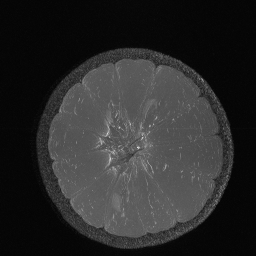
\includegraphics[scale=0.6]{./sortieorange.png}}
\caption{MIP orange}

\centerline{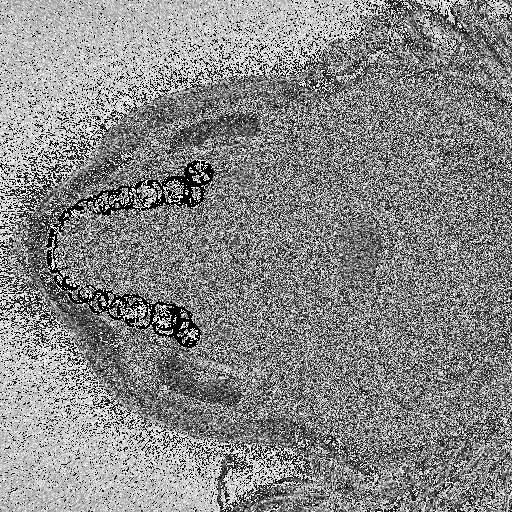
\includegraphics[scale=0.4]{./sortieINCISIX.png}}
\caption{MIP INCISIX}
\end{figure}


\begin{figure}[h]
\centerline{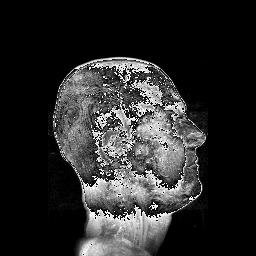
\includegraphics[scale=0.7]{./sortiet1head.png}}
\caption{MIP t1-head}
\end{figure}


\begin{figure}[h]
\centerline{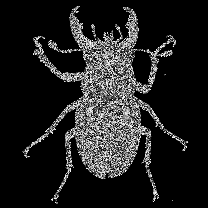
\includegraphics[scale=0.7]{./sortieWhatisit.png}}
\caption{MIP whatisit}
\end{figure}

\newpage
\section{AIP}

\begin{lstlisting}
     for (size_t i = 0; i < dimX; i++)
    {
        for (size_t j = 0; j < dimY; j++)
        {
            int max = 0;
            for (size_t k = 0; k < dimZ; k++)
            {
                // if (getValue(contenu, i, j, k, dimX, dimY, dimZ) < max)
                max += getValue(contenu, i, j, k, dimX, dimY, dimZ);
            }
            max=max/dimZ;
            if(max>255) max=255;
           
            Out[j * dimX + i] = moy ;
        }
    }

\end{lstlisting}



\begin{figure}[h]
\centerline{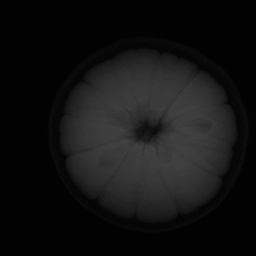
\includegraphics[scale=0.6]{./sortiet1orangemoy.png}}
\caption{AIP orange}

\centerline{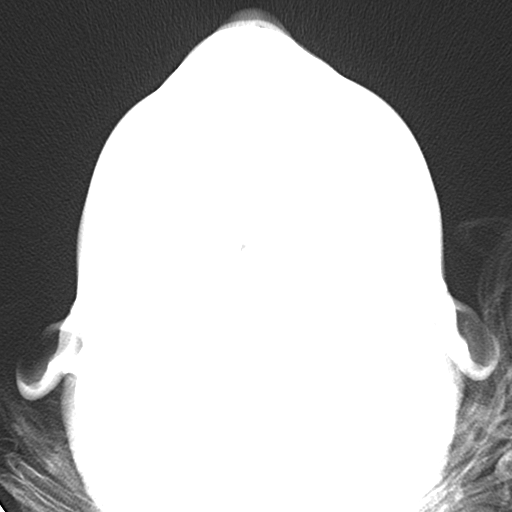
\includegraphics[scale=0.4]{./sortiet1INCISIXmoy.png}}
\caption{AIP INCISIX}
\end{figure}


\begin{figure}[h]
\centerline{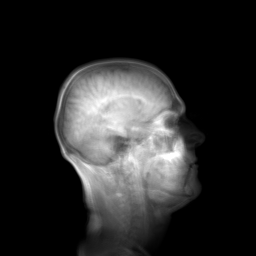
\includegraphics[scale=0.7]{./sortiet1headmoy.png}}
\caption{AIP t1-head}
\end{figure}


\begin{figure}[h]
\centerline{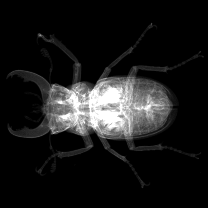
\includegraphics[scale=0.7]{./sortiet1whatisitmoy.png}}
\caption{AIP whatisit}
\end{figure}











\end{document}